\section{Qualità secondo gli standard}
Al fine di perseguire la qualità secondo quanto descritto in questo documento, si è deciso di basarsi su degli standard (descritti qui di seguito) per poter bilanciare la poca esperienza del team con la conoscenza presente in tali documenti, ricavata da anni di pratica nell'ambito dell'ingegneria del software.
\subsection{Standard di processo: ISO/IEC 15504 - Software Process Improvement and Capability Determination}
\label{AppA:standardProc}
%FONTI:
%http://www.plays-in-business.com/isoiec-15504-spice/
La qualità di un prodotto software dipende dalla qualità dei suoi processi. L'\emph{ISO/IEC 15504 - Software Process Improvement and Capability Determination} o \emph{SPICE} è uno standard che permette di valutare i processi software di un prodotto con lo scopo di migliorarli  (in modo continuativo). La valutazione dei processi permette di identificare in modo indipendente la \emph{capacità}\ped{G} (capability) di ciascuno di essi attraverso i loro attributi (ovvero gli esiti della valutazione). Basandoci su tali risultati di valutazione, che devono essere comparabili, ripetibili ed oggettivi, ci si può aspettare un miglioramento \emph{continuativo} dei processi e si possono identificare i loro punti di forza, di debolezza, i rischi ed i modi per prevenirli.

Ad ogni processo viene assegnato un livello di capacità a seconda della classificazione dei suoi attributi:
\begin{labeling}{alligator}
	\item \textbf{0 - incomplete}: il processo presenta una incapacità generale nel raggiungere il proprio obbiettivo. A questo livello di capacità non viene associato alcun attributo;
	
	\item \textbf{1 - performed}: il processo è riuscito a raggiungere il proprio obbiettivo. Il raggiungimento di tale obbiettivo potrebbe non essere stato pianificato e tracciato in modo rigoroso. A questo livello è associto l'attributo \textbf{process performance};
	
	\item \textbf{2 - managed}: il processo (che appartiene anche al livello 1) rilascia i propri prodotti secondo procedure specifiche ed è pianificato e tracciato. I prodotti sono conformi agli standard specificati ed ai requisiti. A questo livello sono associati due attributi: \textbf{performance management} e \textbf{work product management};
	
	\item \textbf{3 - established}: il processo (che appartiene anche al livello 2) viene implementato utilizzando dei buoni principi di ingegneria del software ed è in grado di raggiungere i medesimi risultati ogni volta che viene eseguito. A questo livello sono associati due attributi: \textbf{process definition} e \textbf{process deployment};
	
	\item \textbf{4 - predictable}: il processo (che appartiene anche al livello 3) viene eseguito nella pratica in modo coerente rimanendo dentro ai limiti di controllo che sono stati definiti per raggiungere il suo obbiettivo. Il livello ha associati gli attributi \textbf{process controll} e \textbf{process measurement};
	
	\item \textbf{5 - optimizing}: le performance del processo (che appartiene anche al livello 4) sono ottimizzate in modo continuo per andare incontro agli obbiettivi ed alle necessità (bisogni) di progetto o di business aziendali presenti e futuri. % I processi raggiungono ''ripetiilità'' nel raggiungere gli obbiettivi di business definiti.
	Anche a questo livello sono associati due attributi: \textbf{process innovation} e \textbf{process optimization}.
\end{labeling}

I 9 attributi che servono per misurare la capacità di un processo sono definiti nel seguente modo:
\begin{labeling}{alligator}
	\item \textbf{Process performance}:  è una misura che indica il raggiungimento degli obbiettivi del processo;
	
	\item \textbf{Performance management}: è una misura che indica come sono gestite le performance del processo;%The performance management attribute is a measure of the extent to which the performance of the process is managed
	\item \textbf{Work product management}: è una misura che indica quanto i prodotti del processo siano gestiti in modo appropriato;
	
	\item \textbf{Process definition}: è una misura che indica quanto il processo sia effettivamente impegnato a rispettare gli standard quando produce i propri esiti;
	
	\item \textbf{Process deployment}: è una misura di quanto il processo standard venga diffuso efficacemente per raggiungere i propri risultati;%The process deployment attribute is a measure of the extent to which the standard process is effectively deployed as a defined process to achieve its process outcomes.
	\item \textbf{Process measurement}:  è una misura che indica quanto vengano usate le misurazioni dei risultati  del processo per assicurarsi che le sue  performance supportino il raggiungimento degli obbiettivi aziendali fissati;
	
	\item \textbf{Process control}:  è una misura che dà un'indicazione di quanto il processo sia gestito in modo quantitativo, in modo tale da produrre un processo che sia stabile, capace\footnote{vedere definizione di \emph{capacità}\ped{G}} e prevedibile entro i limiti definiti;%The process control attribute is a measure of the extent to which the process is quantitatively managed to produce a process that is stable, capable, and predictable within defined limits.
	\item \textbf{Process innovation}: è una misura di quanto i cambiamenti apportati al processo siano identificati grazie ad analisi di cause comuni delle variazioni delle performance e da indagini di approcci innovativi per le definizioni e lo sviluppo dei processi;%The process innovation attribute is a measure of the extent to which changes to the process are identified from analysis of common causes of variation in performance, and from investigations of innovative approaches to the definition and deployment of the process 
	\item \textbf{Process optimization}: è una misura che indica quanto i cambiamenti alla definizione, gestione e performance del processo abbiano un impatto effettivo che permetta di raggiungere gli obiettivi rilevanti di miglioramento del processo.%The process optimization attribute is a measure of the extent to which changes to the definition, management and performance of the process result in effective impact that achieves the relevant process improvement objectives
\end{labeling}

Ogni attributo di processo viene valutato attraverso una scala di valutazione di quattro livelli\footnote{Descritti nella parte 3 dello standard}. Il punteggio è basato sulle prove raccolte tramite degli indicatori che permettono di sapere in quale livello della classifica sia posizionato l'attributo. 
\begin{labeling}{alligator}
	\item \textbf{N - Not achieved}: (0\% - 15\%);
	\item \textbf{P - Partially achieved}: (>15\% - 50\%);
	\item \textbf{L - Largely achieved}: (>50\% - 85\%);
	\item \textbf{F - Fully achieved}: (>85\% - 100\%).
\end{labeling}

Per raggiungere un certo livello di capacità, tutti gli attributi di processo del livello in questione devono essere realizzati almeno come "L" e tutti gli attributi di tutti i livelli di capacità sottostanti devono essere "F".

In Figura~\ref{fig:liv_cap_spice} sono rappresentati gli ultimi cinque livelli di capacità dei processi di SPICE ed i relativi attributi ad essi associati.

\begin{figure}[h!]
	\centering
	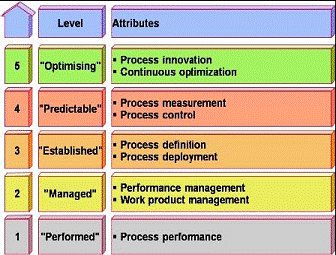
\includegraphics[width=0.50\textwidth]{img/liv_cap_spice.jpg}
	\caption{Ultimi 5 livelli di capacità di SPICE}
	\label{fig:liv_cap_spice}
\end{figure}


\subsection{Standard di prodotto: ISO/IEC 9126}
\label{AppA:standardProd}
Per valutare la qualità del prodotto software si è deciso di utilizzare lo standard ISO/IEC 9126, che è suddiviso in 4 parti:
\begin{labeling}{alligator}
	\item \textbf{Quality Model}: caratteristiche di qualità che possono essere usate per descrivere i fattori di qualità di un prodotto software;
	
	\item \textbf{External Metrics}: metriche non misurabili direttamente che possono essere usate per valutare se il prodotto software è conforme al modello di qualità;
	
	\item \textbf{Internal Metrics}: metriche direttamente misurabili utilizzabili per valutare le external metrics;
	
	\item \textbf{Quality in Use Metrics}: metriche rivolte alla valutazione del sottoinsieme di caratteristiche di qualità legate all’utente.
\end{labeling}

Secondo lo standard sono necessari tre punti di vista per valutare la qualità del prodotto software:
\begin{itemize}
	\item \textbf{Percepita/in uso}: è correlata a ciò che percepisce l'utente e per questo motivo definisce delle metriche che possono essere applicate solamente quando il prodotto è finito. Tali metriche esprimono l'efficacia e l'efficienza con cui il software serve le esigenze del suo utilizzatore;
	 
	\item \textbf{Esterna}: rappresenta le prestazioni del prodotto e le funzionalità che esso offre. Definisce le metriche che esprimono il comportamento dinamico del software e per questo motivo è rilevata attraverso l'analisi dinamica e determina la qualità in uso. È una misura dell'interazione tra il cliente ed il prodotto in un contesto d'uso specifico e permette di osservare il comportamento del software mentre questo viene utilizzato;
	
	\item \textbf{Interna/intrinseca}: rappresenta le qualità intrinseche del prodotto, ovvero quelle misurabili direttamente dal codice sorgente attravero un'analisi di tipo statico. Si realizza partendo dalle specifiche di qualità fornite dall'utente e da quelle tecniche tradotte dallo sviluppatore nell'architettura del software.
\end{itemize}

Gli attributi di qualità interni influenzano alcuni degli attributi di qualità esterni e quest'ultimi influenzano quelli della qualità in uso.

Per descrivere i tre punti di vista di cui sopra, lo standard definisce due modelli, uno che riguarda la qualità interna ed esterna ed un altro che riguarda la qualità in uso. Tali modelli presentano due livelli di caratteristiche (primo e secondo) che definiscono la qualità. Le caratteristiche del secondo livello sono sottocaratteristiche del primo livello e vengono valutate rispetto alle metriche interne ed esterne. In Figura~\ref{fig:int_ext} e in Figura~\ref{fig:in_use} si possono vedere le caratteristiche associate ai due modelli.

\begin{figure}[h!]
	\centering
	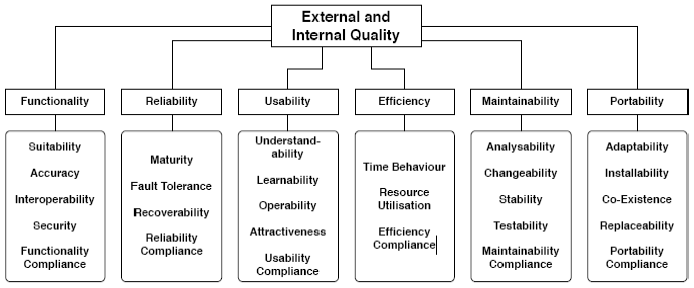
\includegraphics[width=0.50\textwidth]{img/int_ext.png}
	\caption{Caratteristiche associate al modello di qualità interna ed esterna}
	\label{fig:int_ext}
\end{figure}

\begin{figure}[h!]
	\centering
	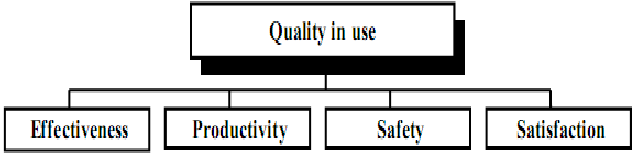
\includegraphics[width=0.50\textwidth]{img/in_use.png}
	\caption{Caratteristiche associate al modello di qualità in uso}
	\label{fig:in_use}
\end{figure}

Di seguito sono elencate le caratteristiche di primo e secondo livello del modello per la qualità interna ed esterna.
\begin{labeling}{alligator}
	\item \textbf{Functionality (funzionalità)}: Il prodotto deve essere in grado di fornire delle funzioni che soddisfino esigenze stabilite (ovvero emerse dall'\AdR{});
	\begin{itemize}
		\item \textbf{Suitability (appropriatezza)}: capacità del prodotto di fornire all'utente delle funzioni in grado di soddisfare le esigenze stabilite ed implicite;
		
		\item \textbf{Accuracy (accuratezza)}: capacità del prodotto di fornire risultati corretti con la precisone richiesta;
		
		\item \textbf{Interoperability (interoperabilità)}: capacità del prodotto di interagire con uno o più sistemi specificati;
		
		\item \textbf{Security (sicurezza)}: capacità del prodotto di proteggere i dati e le informazioni in modo che persone/sistemi non autorizzate/i riescano ad accedervi in lettura o scrittura;
		
		\item \textbf{Compliance (conformità)}: capacità del prodotto di aderire agli standard relativi alle funzionalità che offre.
	\end{itemize}
	\item \textbf{Reliability (affidabilità)}: Il prodotto software deve mantenere un livello di prestazioni specificato quando viene eseguito sotto certe condizioni specificate;
	\begin{itemize}
		\item \textbf{Maturity (maturità)}: capacità del prodotto di evitare anomalie;
		
		\item \textbf{Fault tolerance (tolleranza all'errore)}: capacità del prodotto di mantenere un livello di prestazioni specificato nel caso in cui occorrano anomalie;
		
		\item \textbf{Recoverability (recuperabilità)}: capacità del prodotto di recuperare un livello di prestazioni specificato ed i dati colpiti da malfunzionamenti;
		
		\item \textbf{Compliance (conformità)}: capacità del prodotto di aderire a standard relativi all'affidabilità.
	\end{itemize}
	
	\item \textbf{Usability (usabilità)}: Il prodotto software deve essere compreso ed utilizzato con gradimento dall'utente;
	\begin{itemize}
		\item \textbf{Understandability (comprensibilità)}: il prodotto software permette di far capire all'utente se può essergli utile per dei compiti particolari;
		
		\item \textbf{Learnability (apprendibilità)}: il prodotto è in grado di far apprendere all'utente come utilizzare le proprie applicazioni;
		
		\item \textbf{Operability (operabilità)}: il prodotto permette all'utente di utilizzarlo e di esercitarne il controllo;
		
		\item \textbf{Attactiveness (attrattività)}: la capacità del prodotto di attrarre l'utente suscitandone un certo livello di gradimento;
		
		\item \textbf{Compliance (conformità)}: la capacità del prodotto di aderire agli standard di usabilità.
	\end{itemize}
	
	\item \textbf{Efficency (efficienza)}: Il prodotto sfrutta al massimo e al meglio le risorse di cui necessita per espletare le proprie funzioni;
	\begin{itemize}
		\item \textbf{Time behaviour (comportamento nel corso del tempo)}: capacità del prodotto di fornire un tempo di risposta appropriato quando esegue le proprie funzioni;
		
		\item \textbf{Resource utilisation (utilizzo delle risorse)}: la capacità del prodotto di usare la giusta quantità ed il giusto tipo di risorse quando esegue le proprie funzioni;
		
		\item \textbf{Compliance (conformità)}: capacità del prodotto di soddisfare gli standard relativi all'effecienza.
		
	\end{itemize}
	
	\item \textbf{Maintainability (manutenibilità)}: capacità del prodotto di evolversi nel tempo grazie a delle modifiche o correzioni;
	\begin{itemize}
		\item \textbf{Analysability (analizzabilità)}: la capacità del prodotto di essere analizzato per scovare le cause dei malfunzionamenti;
		
		\item \textbf{Changeability (modificabilità)}: la capacità del prodotto di essere modificato;
		
		\item \textbf{Stability (stabilità)}: capacità del software di evitare malfunzionamenti dopo essere stato modificato;
		
		\item \textbf{Testability (testabilità)}: capacità del software modificato di essere verificato e validato;
		
		\item \textbf{Compliance (conformità)}: capacità del prodotto di soddisfare gli standard relativi alla manutenibilità.
	\end{itemize}
	
	\item \textbf{Portability (portabilità)}: Il software deve poter essere trasferito da un ambiente ad un altro con l'avanzare delle nuove tecnologie.
	\begin{itemize}
		\item \textbf{Adaptability (adattabilità)}: la capacità del prodotto di adattarsi ad ambienti diversi senza che ci sia il bisogno di applicare alcuna azione o di utilizzare mezzi diversi da quelli che sono stati già forniti;
		
		\item \textbf{Installability (instabilità)}: la capacità del prodotto di essere installato in un ambiente specifico;
		
		\item \textbf{Co-existence (coesistenza)}: la capacità del prodotto di coesistere con altri prodotti software indipendenti in uno stesso ambiente condividendone le risorse;
		
		\item \textbf{Replaceability (sostituibilità)}: la capacità del prodotto di sostituire un altro prodotto software con gli stessi scopi nello stesso ambiente;
		
		\item \textbf{Compliance (conformità)}: capacità del prodotto di soddisfare gli standard relativi alla portabilità.
	\end{itemize}
\end{labeling}

Di seguito sono elencate le caratteristiche del modello per la qualità in uso che rappresentano il punto di vista dell'utente sulla qualità del prodotto software:

\begin{itemize}
	\item \textbf{Effectiveness (efficacia)}:  permette agli utenti di raggiungere il proprio obbiettivo portandolo a termine con accuratezza e completezza;

	\item \textbf{Productivity (produttività)}: la capacità del prodotto di utilizzare una adeguata quantità di risorse garantendo efficienza;

	\item \textbf{Satisfaction (soddisfazione)}: la capacità del prodotto software di soddisfare gli utenti;

	\item \textbf{Safety (sicurezza)}: la capacità del prodotto di raggiungere livelli accettabili di rischio di danni a persone, software e ambiente operativo su cui è installato.
\end{itemize}

\subsection{Ciclo di Deming}
Il ciclo di Deming, chiamato anche PDCA (Plan, Do, Check, Act.) è uno strumento che permette di realizzare il miglioramento continuo della qualità dei processi e quindi anche dei loro prodotti.

\begin{figure}[h!]
	\centering
	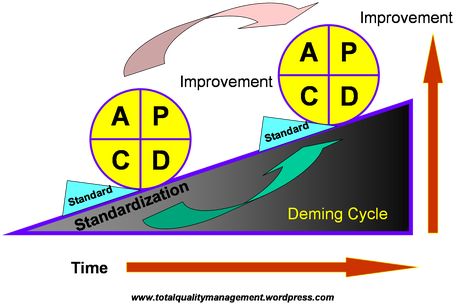
\includegraphics[width=0.50\textwidth]{img/deming.png}
	\caption{Ciclo di Deming}
	\label{fig:PDCA}
\end{figure}

Come si può vedere in Figura~\ref{fig:PDCA} bisogna ripetere in modo iterativo i quattro passi \emph{Plan}, \emph{Do}, \emph{Check} e \emph{Act} per ottenere il miglioramento di un processo.

\begin{itemize}
	\item \textbf{Plan}: vengono pianificati gli obbiettivi per il miglioramento del processo. In questa fase viene analizzata la situazione attuale, vengono raccolti i dati e sviluppate delle metodologie per ottenere dei miglioramenti. Vengono definite le attività che bisogna svolgere, le risorse di cui esse necessitano e si fissano le scadenze.
	
	Per fare ciò è necessario porsi tre domande durante la fase di planning:
	\begin{itemize}
		\item Cosa si sta cercando di realizzare?
		\item Quali cambiamenti si possono fare per ottenere un miglioramento?
		\item Come si è in grado di capire che un dato cambiamento rappresenta un miglioramento?
	\end{itemize}

	\item \textbf{Do}: viene attuato il piano definito nella fase di Plan, in questo modo il processo viene eseguito e così viene creato il prodotto;
	
	\item \textbf{Check}: viene controllato che il processo funzioni come pianificato, in particolare si confrontano i risultati misurati nella fase di Do con gli obbiettivi stabiliti nella fase di Plane (ovvero i risultati attesi);
	
	\item \textbf{Act}: il processo viene migliorato attuando se necessario delle azioni correttive che devono agire sulle differenze riscontrate tra i risultati attesi e quelli misurati.
\end{itemize}

Quando tutte queste quattro fasi vengono portate a termine con il massimo della soddisfazione, il miglioramento viene standardizzato. Il prodotto standardizzato è il risultato dell'iniziativa di miglioramento. É possibile che con il cambiamento di alcune circostanze, il processo sia soggeto ad un nuovo miglioramento, in questo modo il ciclo di deming viene ripetuto di volta in volta.